\documentclass[a4paper]{article}
%\documentclass[a4paper,10pt]{article}
\usepackage{geometry}
 \geometry{
 a4paper,
 total={210mm,297mm},
 left=20mm,
 right=20mm,
 top=20mm,
 bottom=20mm,
 }
\usepackage[utf8]{inputenc}
\usepackage[english]{babel}
\usepackage{makeidx}
\usepackage{url}
\usepackage{tikz}
\usepackage{float}
\usepackage{pdfpages}
\usepackage{amsfonts}
\usepackage{mdwlist}
\usepackage{xcolor}
\usepackage{listings}
\usepackage[utf8]{inputenc}
\usepackage[T1]{fontenc}
\usepackage{listingsutf8}
\usepackage{cite}
\usepackage{amsmath}
\usepackage{mdframed}
\usepackage[affil-it]{authblk}

\begin{document}
\title{Basic Pollard Rho Algorithm Implementation On \texttt{CUDA} Device}
\author{Martin Beránek}
\date{\today}
\affil{Faculty of Information Technology -- Czech Technical University in Prague}
\maketitle

\tableofcontents
\listoffigures
%\listoftables
\newpage

\section{Introduction}

The factorisation problem of a huge number resolved into massive parallel solutions. A Large number of algorithms are currently state-of-art and are continuously developed into better forms. This short article is focused on implementation of the Pollard-Rho algorithm on \texttt{CUDA} device. In the first part, there is a definition of algorithm. Next, the article focuses on options of parallelism on CUDA device. Results are measured in multiple instances and compared in graphs. 

\section{Definition of the algorithm}

The $\rho$ algorithm (named after the shape of curves symbolising two functions trying to reach themselves in the projective space) is based on finding the cycle. In $t$ random numbers of $x_1, x_2, \dots, x_t$ in range $[1, n]$ will contain repetition with probability of $P > 0.5$ if $t > 1.777n^{\frac{1}{2}}$

The $\rho$ algorithm uses $g(x)$ with modulo $n$ as a generator for pseudo-random sequence. In this article function $x^2 + k;\, k \in \mathbb{N}$. We are assuming that $n = p \cdot q$ that also mean $p < \sqrt{n}$ and $q < \sqrt{n}$. Algorithm actually generates sequence of $x_1 = g(2),\,x_2 = g(g(2)),\,\dots$ in two separated sequences running in same time. One sequence is generated as $x_1=g(x_0) \mod n$ and second as $x_1=g(g(x_0)) \mod n$. Since we know that $p < \sqrt{n}$ the faster sequence is likely to cycle faster then the sequence generated just in in application of a $g$ function. The repetition of the $\mod p$ will be detected with $| x_k - x_m |$ which will divide $p$ without any residue \cite{wiki}.

\begin{figure}[H]
    \centering
    \begin{lstlisting}
    x=2; y=2; d=1
    while d is 1:
        x = g(x)
        y = g(g(y))
        d = gcd(|x - y|, n)
        if d = n: 
            return failure
        else:
            return d
    \end{lstlisting}
    \caption{Sequential pseudo-code of algorithm}
    \label{singl_alg}
\end{figure}

While the implementation in \texttt{Python} is basically just a copy of pseudo-code, in \texttt{C} there is plenty struggle with fix size integer size. Another problem will be with the transformation of libraries like \texttt{GNU MP}, that's why the basic focus on sequential solution was on basic mathematical operations. For the basic adding and subtracting there was no bigger effort than just creating basic implementation with carry bits. Much more time was spent on operations like division and modulo.

\subsection{Division}

The first idea on how to divide numbers was to use school \emph{Long division} algorithm which proved to be a little bit expensive but was behaving in the same manners for every input numbers.

\begin{figure}[H]
    \centering
    \begin{lstlisting}
Q = 0
R = 0                     
for i = n - 1 .. 0 do
    R = R << 1
    R(0) = N(i)
    if R >= D then
        R = R - D
        Q(i) = 1
    \end{lstlisting}
    \caption{Long division \cite{long_div}}
    \label{long_div}
\end{figure}

Another much faster division was to use \emph{Knuth's division} \cite{knuth} which took a considerably shorter time to compute. Yet there was no luck in implementation. Current version which was considered is from \texttt{llvm} \cite{llvm}. But it failed with some badly shifted bits in residuum hence was not used.

\subsection{\texttt{GCD}}

Since the division wasn't fast enough, at least \texttt{GCD} was implemented with shifts and small bit checks. This may lead to more divergent behaviour in \texttt{CUDA} implementation.

\begin{figure}[H]
    \centering
    \begin{lstlisting}[language=c,basicstyle=\small]
__device__  inline void gcd(unsigned int * A, unsigned int * B){
    unsigned int t [SIZE];
    unsigned int shift;

    if(zeroNum(B)){
        return;
    }
    if(zeroNum(A)){
        copyNum(A, B);
        return;
    }
    for(shift = 0; ((A[0] | B[0]) & 1) == 0; ++ shift){
        shiftRightNum(A);
        shiftRightNum(B);
    }
    while((A[0] & 1) == 0){
        shiftRightNum(A);
    }
    do{
        while((B[0] & 1) == 0){
            shiftRightNum(B);
        }
        if(bigger(A, B) == 1){
            copyNum(t, B);
            copyNum(B, A);
            copyNum(A, t);
        }
        subNum(B, A);
    } while (! zeroNum(B));
    shiftLeftNumBy(A, shift);
}
    \end{lstlisting}
    \caption{\texttt{GCD} algorithm}
    \label{gcd}
\end{figure}

\subsection{Measurements}

To make some basic idea on how fast the algorithm is, there was picked large number composed with big prime numbers $N = 0x0fd42d4eb2c4b7b1 = 1140586421661513649 = 1067982407 \cdot 1067982407$. Whole run of sequential implementation shows that there is only $54443$ iterations to finish the task.


\begin{figure}[H]
    \centering
    \begin{lstlisting}[language=sh,basicstyle=\small]
********************

real    0m3.081s
user    0m3.072s
sys    0m0.000s
    \end{lstlisting}
    \caption{Command time output on sequential run}
    \label{tmsq}
\end{figure}

\texttt{CPU} which was used was \texttt{AMD Phenom(tm) II X4 960T Processor}.

\section{\texttt{CUDA} Solution}


\subsection{First solution with explicit barrier}

First idea which was found at \url{https://github.com/dghost/factor-cuda}. Implementation prepared at host memory $X, Y, C$ for the algorithm which was, later on, ran with multiple kernels and explicitly synchronised after each loop. For the parameters $X, Y, C$ were used random numbers which could let to same sequences. From this, there was an easy step to create deterministic $X, Y, C$ just by giving them numbers from 1 till the number of running threads. This actually led to creating a kernel which prepared data directly at the global memory of device without the need of host \texttt{CPU}. Algorithm work as follow:

\begin{figure}[H]
    \centering
    \begin{lstlisting}

    create R variable which should, later on, contain the result

    copy input N to the device memory space

    call kernel which creates input variables X, Y, C
        for each thread in each block

    while R is zero:
        
        call kernel which is one iteration of Pollard Rho cycle

        copy R from device to host memory space

    \end{lstlisting}
    \caption{First version of Pollard-Rho on \texttt{CUDA}}
    \label{gcd}
\end{figure}

The whole approach is based not on dividing the cycle into same size small problems but rather trying different starting positions and hoping some of them reach the result much faster. That would mean the algorithm could be in the worst case as same fast as the implementation in the single thread.

\subsection{Measurements}

For measurement in this case was chose small number:

\begin{verbatim}
N[0] = 0xb2c4b7b1;
N[1] = 0x0fd42d4e;
\end{verbatim}

The number is really small and at the most complex operation like a power of two, it would take about 5 times 32 bits. That would also raise a question of bank conflicts. Yet with using a huge number of blocks and threads, this wouldn't need to be a problem. Another change was to force using \texttt{L1} cache. Since number size is not huge, caching could provide huge speed up.

 
\begin{figure}[H]
    \centering
    \begin{lstlisting}
cudaFuncSetCacheConfig(prepareDataKernel, cudaFuncCachePreferL1);
cudaFuncSetCacheConfig(pollardKernel, cudaFuncCachePreferL1);
    \end{lstlisting}
    \caption{Changing caching policy for both kernels}
    \label{llcache}
\end{figure}

With that, the average time of execution was about $11505.4$ [ms]. Graph of all runs does not show any significant speed up in a particular number of blocks and number of threads. Only large slow down at blocks size of 10 with 10 threads which is obvious.

\begin{figure}[H]
  \centering
    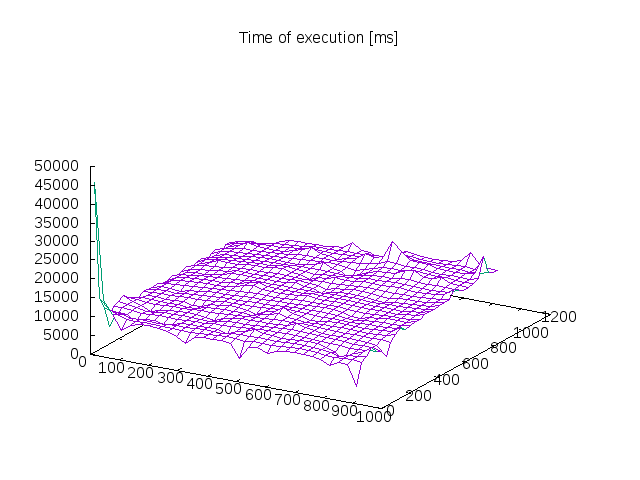
\includegraphics[width=0.8\textwidth]{graph_v1.png}
  \caption{Graph of execution time}
  \label{exec}
\end{figure}

Some small speedups were noticed in cases where particular input $X, Y, C$ were given. In these cases, the algorithm could end much faster because of simple luck of choosing good input. From opposite point of view, some cases were so unlucky with choosing initial values that some small slow downs were noticed as well.

\subsubsection{Profiler output}

Profiling was done on \texttt{NVidia GeForce GTX 780 Ti} at \texttt{gpu-02.star.fit.cvut.cz}.

Another problem would maybe occur in the divergence of threads in \texttt{warp}. The algorithm works with non-native mathematical operations which are used for big numbers. With big probability, the divergences occur at modulo operation. Because of large usage of \texttt{while} in \texttt{GCD} the operation could also cause a lot of divergences as well. For this reasons, profiler testing is provided showing about $50\%$ of the runtime is given to waiting.

\begin{figure}[H]
  \centering
    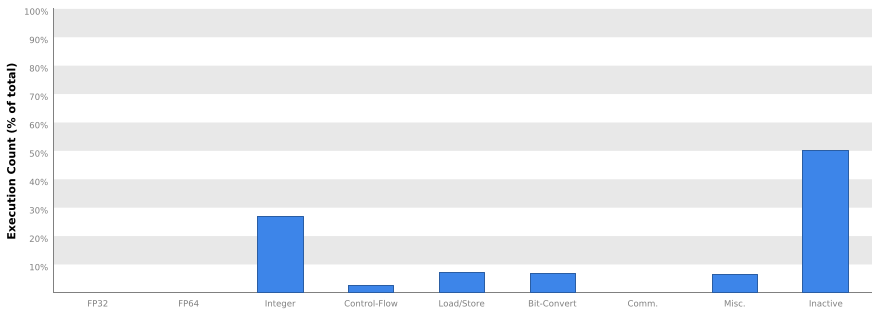
\includegraphics[width=1\textwidth]{inactive.png}
  \caption{Inactivity of threads in \texttt{warp}}
  \label{inactive}
\end{figure}


There are further indications of efficiency. Profiler provided the count of instructions which were used:

\begin{figure}[H]
  \centering
    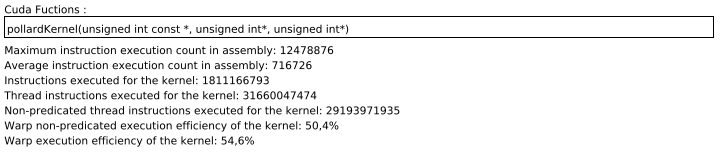
\includegraphics[width=0.8\textwidth]{insv1.png}
  \caption{Count of instructions used by kernels}
  \label{inactive}
\end{figure}

Some other techniques were used. For example \texttt{\_\_restrict\_\_} was given to data pointers and \texttt{const} was added to $N$ which is untouched in the whole algorithm. Yet the biggest problem of diverging threads in warp wasn't fully solved.

For further detail see \url{pollardKernel_v1.pdf}.

\subsection{Second solution with independent runners}

Another idea was to omit using global memory at all. So the threads would run algorithm from different input values $X, Y, C$ and after some time each one of them would check if the there is some result. If some thread found solution whole algorithm stop.

% awk 'BEGIN{lns=0;total=0;}{lns ++; total += $3;}END{print total/lns;}' data_v2.txt 
% 488627

\begin{figure}[H]
    \centering
    \begin{lstlisting}[language=c,basicstyle=\small]

__global__ void pollardKernel(const unsigned int * N, unsigned int * result){
    unsigned int threadID = blockIdx.x * blockDim.x + threadIdx.x;
    unsigned int X[SIZE];
    unsigned int Y[SIZE];
    unsigned int C[SIZE];
    unsigned int G[SIZE];
    unsigned int N_tmp[SIZE];
    unsigned int abs_mxy[SIZE];
    
    cuda_setZero(X);
    X[0] = 0x07;
    cuda_setZero(C);
    C[0] = threadID + 1;
    cuda_setZero(G);
    G[0] = 0x01;
    cuda_copyNum(Y, X);
    cuda_fxfun(N, Y, C);
   
    unsigned int check = 0;

    while (cuda_isOne(G)){
        cuda_fxfun(N, X, C);
        cuda_fxfun(N, Y, C);
        cuda_fxfun(N, Y, C);
        if(cuda_bigger(X, Y) == 1){
            cuda_copyNum(abs_mxy, X);
            cuda_subNum(abs_mxy, Y);
        }else{
            cuda_copyNum(abs_mxy, Y);
            cuda_subNum(abs_mxy, X);    
        }
        cuda_copyNum(G, abs_mxy);
        cuda_copyNum(N_tmp, N);
        cuda_gcd(G, N_tmp);
        check ++;
        if ((check % (100) == 0) && !cuda_zeroNum(result)){
            return;
        }
    }
    
    cuda_copyNum(result, G);    
}

    \end{lstlisting}
    \caption{Kernel from second version}
    \label{kernelv2}
\end{figure}

As you can see, after every 100 iteration thread check if some other thread hasn't solved the problem and stop. 


\subsection{Measurements}

For measurement in this case was chossen small number:

\begin{verbatim}
N[0] = 0xb2c4b7b1;
N[1] = 0x0fd42d4e;
\end{verbatim}

Again, the policy of preferring \texttt{L1} was used. There was much less memory access since there is none global memory used. The only thing regarding bank conflict could be in accessing result which is actually provided to other threads as broadcast.

The average time of execution was $488627$ [ms] which is much higher than in the last case.

\begin{figure}[H]
  \centering
    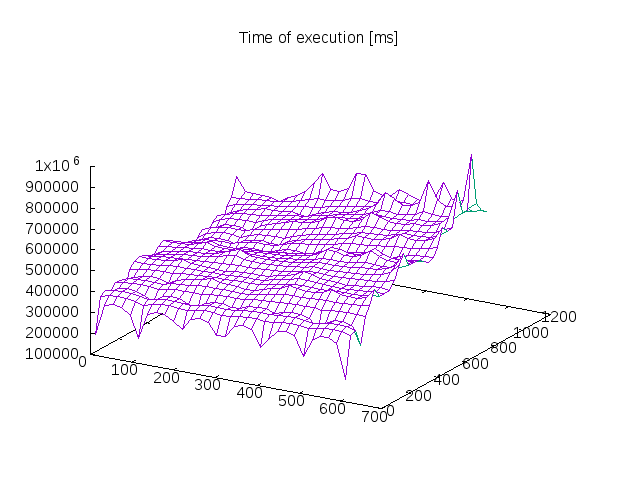
\includegraphics[width=0.8\textwidth]{graph_v2.png}
  \caption{Graph of execution time}
  \label{exec2}
\end{figure}

From this graph, we can observe that execution time is much higher.

\subsubsection{Profiler output}

Profiling was done on \texttt{NVidia GeForce GTX 780 Ti} at \texttt{gpu-02.star.fit.cvut.cz}.

In this case, the profiler didn't provide that much date with an explanation that it couldn't obtain them. Even after changing initial input value of $N$ the profiler wasn't able to generate some result. But at least the ratio of which instructions were used was given. That actually showed how much diverged the algorithm was during the run.

\begin{figure}[H]
  \centering
    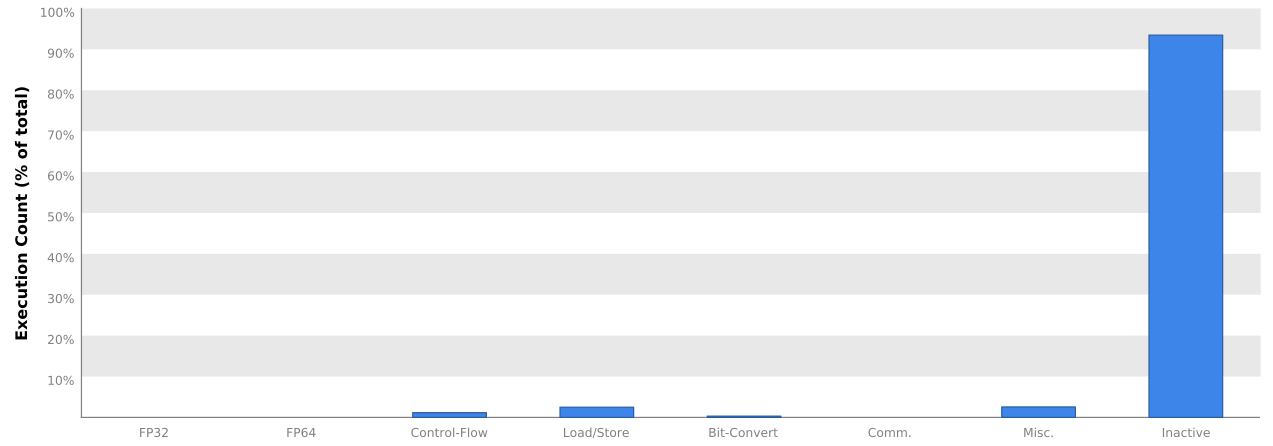
\includegraphics[width=1\textwidth]{inactive2.png}
  \caption{Inactivity of threads in \texttt{warp}}
  \label{inactive2}
\end{figure}

As the chart shows, divergence in this solution is huge, making it unusable for any usable results. A much worst case could appear with using bigger numbers.

\section{Conclusion}

The whole \texttt{CUDA} solution is based on pure luck finding some input values which actually converge faster to find some number dividing input $N$. To make the algorithm more deterministic, there is no random function used to fill input values. If random would be used, some threads could actually by some small probability count the same sequence. But on the other hand, some threads could converge much faster. \texttt{CUDA} contain library which can provide random numbers \texttt{cuRAND} \cite{cuRAND} which have big throughput, therefore there is no need to generate random numbers on host \texttt{CPU}.

In this solutions first \texttt{CUDA} implementation won. To compare for the same input $N$ the speed up was $5.52$ times. But! We have to notice that we picked block size $810$ with a thread count $110$. This solution was found with measuring going from $1$ to $1024$ for both block and thread count. Therefore, for new generic input number $N$ there would be most strategic to get this numbers as big as local $SM$ can serve.

Another much-needed improvement would be to work with some kind of \texttt{GMP} library which would contain a much better implementation of basic mathematical operations. Since this article is not about creating the fastest way to compute these operations, there is much to be done to improve them. With that, there should be some kind of relation with \texttt{CUDA} devices. If the number is big enough to rotate in memory banks, conflicts can occur making the whole implementation much slower. Same thing applies to the divergence of threads which was so much obvious in this implementation. If the mathematical operations would just work without any ifs and whiles, there should be much-needed speed up.


\bibliographystyle{iso690}
\bibliography{mybibliographyfile}


\end{document}
